%% This is a skeleton file demonstrating the advanced use of IEEEtran.cls
%% (requires IEEEtran.cls version 1.8b or later) with an IEEE Computer
%% Society journal paper.

\documentclass[10pt,journal,compsoc]{IEEEtran}

\usepackage[nocompress]{cite}

\usepackage[pdftex]{graphicx}
\graphicspath{{./jpeg/}}
\DeclareGraphicsExtensions{.pdf,.jpeg,.png}

\usepackage{amsmath}
\usepackage[listings,skins]{tcolorbox}
\interdisplaylinepenalty=2500

\newcommand\MYhyperrefoptions{bookmarks=true,bookmarksnumbered=true,
pdfpagemode={UseOutlines},plainpages=false,pdfpagelabels=true,
colorlinks=true,linkcolor={black},citecolor={black},urlcolor={black},
pdftitle={Bare Demo of IEEEtran.cls for Computer Society Journals},%<!CHANGE!
pdfsubject={Typesetting},%<!CHANGE!
pdfauthor={Michael D. Shell},%<!CHANGE!
pdfkeywords={Computer Society, IEEEtran, journal, LaTeX, paper,
             template}}%<^!CHANGE!

\hyphenation{op-tical net-works semi-conduc-tor}

\usepackage{polski}
\usepackage[utf8]{inputenc}
\renewcommand\IEEEkeywordsname{Słowa kluczowe}

\begin{document}
\title{Rozszerzenie Programowe RNS Procesora x86 \\ Mnożenie Montgomerego}

\author{Jan~Jurec,~\IEEEmembership{Student,~PWR,}
        Filip~Toruń,~\IEEEmembership{Student,~PWR}}

\markboth{sprawozdanie z projektu z organizacji i architektury komputerów, Czerwiec~2017}%
{Shell \MakeLowercase{\textit{et al.}}: sprawozdanie z projektu z organizacji i architektury komputerow, Czerwiec~2017}
% The only time the second header will appear is for the odd numbered pages
% after the title page when using the twoside option.

% Justowanie abstraktu
\makeatletter
\long\def\@IEEEtitleabstractindextextbox#1{\parbox{0.922\textwidth}{#1}}
\makeatother

\IEEEtitleabstractindextext{
\begin{abstract}
Kryptografia jest jedną z najszybciej rozwijających się i najbardziej kluczowych dziedzin informatyki. Skuteczne zaszyfrowanie danych pozwala na bezpieczne ich przechowywanie oraz wymianę choćby w systemach bankowych czy prywatnych rozmowach. Do najbezpieczniejszych systemów kryptograficznych należą kryptosystemy asymetryczne, wśród których bardzo popularne są algorytmy RSA i Diffiego-Hellmana. Oba oparte są na operacjach modularnej na wielkich liczbach, która jest niezwykle kosztowna. Ten artykuł pokazuje drogę, jaką przeszli autorzy, by zbliżyć się do zrozumienia  działania mnożenia~Montgomerego - algorytmu, który znacznie zmniejsza koszt obliczeń w arytmetyce modulo. 
\end{abstract}

\begin{IEEEkeywords}
System Resztowy, Chińskie Twierdzenie o Resztach, Systemy Liczbowe, Arytmetyka Komputerowa, Orgainizacja i Architektura Komputerów, Piotr Patronik Projekt, Mnożenie Montgomerego, Kryptografia, Optymalizacja 
\end{IEEEkeywords}}


\maketitle


\IEEEdisplaynontitleabstractindextext
\IEEEpeerreviewmaketitle


\IEEEraisesectionheading{\section{WSTĘP}\label{sec:wstęp}}
\IEEEPARstart{A}{by} zrozumieć działanie mnożenia Montgomerego należy najpierw poznać własności systemu resztowego i zrozumieć, jak przebiegają w nim operacje. W tym celu autorzy zaimplementowali konwersję w przód i w tył, używając chińskeigo twierdzenia o resztach. Później napisali również dodawanie, odejmowanie, mnożenie oraz dzielenie przez potęgę liczby 2 w systemie resztowym dla liczby 32-bitowej w systemie modułów 7, 15, 31, 127, 8192. Rezultat tych zmagań, które zajęły większą część czasu projektu udostępniają autorzy w Dodatku A. Po zapoznaniu się z arytmetyką modularną autorzy przystąpili do implementacji algorytmu mnożenia Montgomerego w samodeskryptywnym języku skryptowym Python. Wynikowy kod udostępniają w Dodatku B. Własności mnożenia w systemie resztowym zauważone przez Piotra Montgomerego pozwalają na drastyczne przyspieszenie multiplikacji a tym samym podnoszenia do potęgi w tymże systemie. Dodatkowo, odpowiednio dobierając parametry systemu modulo, można jeszcze bardziej usprawnić obliczenia wykorzystując natychmiastowość dzielenia oraz uzyskiwania reszty z dzielenia przez potęgi liczby 2 w komputerach ogólnego zastosowania.\\\\\\

\IEEEraisesectionheading{\section{Metoda Separated Operand Scanning}\label{sec:metoda1}}
\IEEEPARstart{P}{ierwszą} metodą analizowaną przez nas była metoda Separated Operand Scanning. Postępuje ona zgodnie z przedstawionym powyżej schematem i dzieli się na 3 kroki.
Pierwszy krok wygląda następująco:
\begin{lstlisting}
for i=0 to s-1
  C := 0
    for j=0 to s-1
      (C,S) := t[i+j] + a[j]*b[i] + C
      t[i+j] := S
    t[i+s] := C
\end{lstlisting}

\noindent Przy czym dodać trzeba, że tablica t musi być wyzerowana, będzie mieć ona długość 2s słów.\\ Krok drugi: 
\begin{lstlisting}
for i=0 to s-1
  C := 0
  m := t[i]*n'[0] mod W
  for j=0 to s-1
    (C,S) := t[i+j] + m*n[j] + C
    t[i+j] := S
  ADD (t[i+s],C)
for j=0 to s
  u[j] := t[j+s]
\end{lstlisting}

\noindent Tutaj naszym produktem jest tablica $u$ o długości s+1 słów. Wartym nadmienienia jest, że korzystamy z $n'[0]=n'\ mod\ 2^w$ $-$ najmniej znaczący bit 
odwrotności multiplikatywnej z~r-n. Funkcja ADD propaguje zadane przeniesienie na bardziej znaczące słowa.

\noindent Ostatni krok powtarza się w obu omawianych metodach. I jest to zwykłe porównanie $u$ z $n$ i zwrócenie $u-n$ gdy $u$ jest większe, a w przeciwnym wypadku zwracamy po prostu $u$.
\begin{lstlisting}
B := 0
for i=0 to s-1
  (B,D) := u[i] - n[i] - B
  t[i] := D
(B,D) := u[s] - B
t[s] := D
if B = 0 then return t[0],t[1],...t[s-1]
	 else return u[0],u[1],...u[s-1]
\end{lstlisting} 
\noindent Ten krok zwraca nam już wynik.\\ \\ \\ \\
\IEEEraisesectionheading{\section{Metoda Coarsely Integrated Operand Scanning}\label{sec:metoda2}}
\IEEEPARstart{D}{ruga} metoda integruje krok pierwszy oraz drugi, dzięki czemu zmniejszone jest zapotrzebowanie na pamięć. Integracja ta polega na wykorzystaniu zewnętrznej pętli do obu operacji - mnożenia oraz redukcji. Jest to możliwe ponieważ $m[i]$ zależne jest jedynie od $t[i]$.
\begin{lstlisting}
for i = 0 to s - 1
  C := 0
  for j = 0 to s - 1
    (C,S) := t[j] + a[j]b[i] + C
    t[j] := S
  (C,S) := t[s] + C
  t[s] := S
  t[s + 1] := C
  C := 0
  m := t[0]n'[0] mod W
  for j = 0 to s - 1
    (C,S) := t[j] + mn[j] + C
    t[j] := S 
    (C,S) := t[s] + C
    t[s] := S
    t[s + 1] := t[s + 1] + C
    for j = 0 to s
      t[j] := t[j + 1]
\end{lstlisting} 
\noindent Znowu tablica $t$ musi być wyzerowana na starcie.
% An example of a floating figure using the graphicx package.
% Note that \label must occur AFTER (or within) \caption.
% For figures, \caption should occur after the \includegraphics.
% Note that IEEEtran v1.7 and later has special internal code that
% is designed to preserve the operation of \label within \caption
% even when the captionsoff option is in effect. However, because
% of issues like this, it may be the safest practice to put all your
% \label just after \caption rather than within \caption{}.
%
% Reminder: the "draftcls" or "draftclsnofoot", not "draft", class
% option should be used if it is desired that the figures are to be
% displayed while in draft mode.
%
%\begin{figure}[!t]
%\centering
%\includegraphics[width=2.5in]{myfigure}
% where an .eps filename suffix will be assumed under latex, 
% and a .pdf suffix will be assumed for pdflatex; or what has been declared
% via \DeclareGraphicsExtensions.
%\caption{Simulation results for the network.}
%\label{fig_sim}
%\end{figure}

% Note that the IEEE typically puts floats only at the top, even when this
% results in a large percentage of a column being occupied by floats.
% However, the Computer Society has been known to put floats at the bottom.


% An example of a double column floating figure using two subfigures.
% (The subfig.sty package must be loaded for this to work.)
% The subfigure \label commands are set within each subfloat command,
% and the \label for the overall figure must come after \caption.
% \hfil is used as a separator to get equal spacing.
% Watch out that the combined width of all the subfigures on a 
% line do not exceed the text width or a line break will occur.
%
%\begin{figure*}[!t]
%\centering
%\subfloat[Case I]{\includegraphics[width=2.5in]{box}%
%\label{fig_first_case}}
%\hfil
%\subfloat[Case II]{\includegraphics[width=2.5in]{box}%
%\label{fig_second_case}}
%\caption{Simulation results for the network.}
%\label{fig_sim}
%\end{figure*}
%
% Note that often IEEE papers with subfigures do not employ subfigure
% captions (using the optional argument to \subfloat[]), but instead will
% reference/describe all of them (a), (b), etc., within the main caption.
% Be aware that for subfig.sty to generate the (a), (b), etc., subfigure
% labels, the optional argument to \subfloat must be present. If a
% subcaption is not desired, just leave its contents blank,
% e.g., \subfloat[].


% An example of a floating table. Note that, for IEEE style tables, the
% \caption command should come BEFORE the table and, given that table
% captions serve much like titles, are usually capitalized except for words
% such as a, an, and, as, at, but, by, for, in, nor, of, on, or, the, to
% and up, which are usually not capitalized unless they are the first or
% last word of the caption. Table text will default to \footnotesize as
% the IEEE normally uses this smaller font for tables.
% The \label must come after \caption as always.
%
%\begin{table}[!t]
%% increase table row spacing, adjust to taste
%\renewcommand{\arraystretch}{1.3}
% if using array.sty, it might be a good idea to tweak the value of
% \extrarowheight as needed to properly center the text within the cells
%\caption{An Example of a Table}
%\label{table_example}
%\centering
%% Some packages, such as MDW tools, offer better commands for making tables
%% than the plain LaTeX2e tabular which is used here.
%\begin{tabular}{|c||c|}
%\hline
%One & Two\\
%\hline
%Three & Four\\
%\hline
%\end{tabular}
%\end{table}


% Note that the IEEE does not put floats in the very first column
% - or typically anywhere on the first page for that matter. Also,
% in-text middle ("here") positioning is typically not used, but it
% is allowed and encouraged for Computer Society conferences (but
% not Computer Society journals). Most IEEE journals/conferences use
% top floats exclusively. 
% Note that, LaTeX2e, unlike IEEE journals/conferences, places
% footnotes above bottom floats. This can be corrected via the
% \fnbelowfloat command of the stfloats package.




\section{Conclusion}
The conclusion goes here.





% if have a single appendix:
%\appendix[Proof of the Zonklar Equations]
% or
%\appendix  % for no appendix heading
% do not use \section anymore after \appendix, only \section*
% is possibly needed

% use appendices with more than one appendix
% then use \section to start each appendix
% you must declare a \section before using any
% \subsection or using \label (\appendices by itself
% starts a section numbered zero.)
%


\appendices
\section{Podstawowe operacje RNS w ASM~AT\&T}
TODO: KOD Z CRT.S TUTAJ

% you can choose not to have a title for an appendix
% if you want by leaving the argument blank
\section{Mnożenie Montgomerego SOS i CIOS w Pythonie}
TODO: KOD Z MONPRO.PY TUTAJ


\section*{Podziękowanie}

Jan Jurec pragnie podziękować swojej narzeczonej Katarzynie za nieustanne wsparcie w uprawianiu nauki, pomoc w ciężkich chwilach i pyszne obiady, które dostarczają mu energii i motywacji do zgłębiania tajników organizacji i arytmetyki komputerów.
Filip Toruń ... TODO: DOPISAĆ
Obaj zaś dziękują Doktorowi Piotrowi Patronikowi, który dzielił się swoją wiedzą i skutecznie motywował do skutecznego przeprowadzenia projektu.

% Can use something like this to put references on a page
% by themselves when using endfloat and the captionsoff option.
\ifCLASSOPTIONcaptionsoff
  \newpage
\fi



% trigger a \newpage just before the given reference
% number - used to balance the columns on the last page
% adjust value as needed - may need to be readjusted if
% the document is modified later
%\IEEEtriggeratref{8}
% The "triggered" command can be changed if desired:
%\IEEEtriggercmd{\enlargethispage{-5in}}

% references section

% can use a bibliography generated by BibTeX as a .bbl file
% BibTeX documentation can be easily obtained at:
% http://mirror.ctan.org/biblio/bibtex/contrib/doc/
% The IEEEtran BibTeX style support page is at:
% http://www.michaelshell.org/tex/ieeetran/bibtex/
%\bibliographystyle{IEEEtran}
% argument is your BibTeX string definitions and bibliography database(s)
%\bibliography{IEEEabrv,../bib/paper}
%
% <OR> manually copy in the resultant .bbl file
% set second argument of \begin to the number of references
% (used to reserve space for the reference number labels box)
\begin{thebibliography}{1}

\bibitem{IEEEhowto:kopka}
H.~Kopka and P.~W. Daly, \emph{A Guide to {\LaTeX}}, 3rd~ed.\hskip 1em plus
  0.5em minus 0.4em\relax Harlow, England: Addison-Wesley, 1999.

\end{thebibliography}

% biography section
% 
% If you have an EPS/PDF photo (graphicx package needed) extra braces are
% needed around the contents of the optional argument to biography to prevent
% the LaTeX parser from getting confused when it sees the complicated
% \includegraphics command within an optional argument. (You could create
% your own custom macro containing the \includegraphics command to make things
% simpler here.)
\begin{IEEEbiography}[{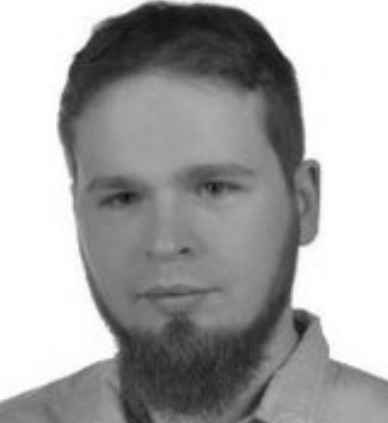
\includegraphics[width=1in,height=1.25in,clip,keepaspectratio]{jjjurec}}]{Jan Jakub Jurec}
Jan Jakub Jurec jest po raz trzeci studentem trzeciego roku Politechniki Wrocławskiej wydziału Elektroniki kierunku Informatyka. Marzeniem autora jest zdanie kursu Organizacja i Architektura Komputerów za trzecim podejściem, bo (jak to drzewiej mawiano) "do trzech razy sztuka"! \\
E-mail: jurec@protonmail.com
\end{IEEEbiography}


\begin{IEEEbiography}[{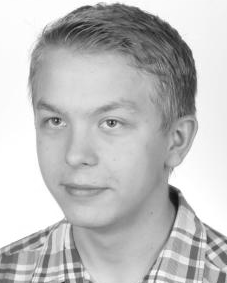
\includegraphics[width=1in,height=1.25in,clip,keepaspectratio]{ftorun}}]{Filip Torun}
Jest studentem Politechniki Wrocławskiej wydziału Elektroniki kierunku Informatyka. \\
E-mail: 209428@student.pwr.edu.pl
\end{IEEEbiography}

%\vfill
%\enlargethispage{-5in}

\end{document}


